%%%%%%%%%%%%%%%%%%%%%%%%%%%%%%%%%%%%%%%%%%%%%%%%%%%%%%%%%%%%%%%%%%%%%%
% Lớp 11 | Giới hạn. Hàm số liên tục | Hàm số liên tục
% Dạng 1D3?3-6: Toán thực tế áp dụng hàm số liên tục
% Số câu: 12  (sinh tự động bởi tach_cau.py; từ nay thầy sửa trực tiếp file này)
%%%%%%%%%%%%%%%%%%%%%%%%%%%%%%%%%%%%%%%%%%%%%%%%%%%%%%%%%%%%%%%%%%%%%%

%%%%%%%%%%%%%%%% TRẮC NGHIỆM 4 PHƯƠNG ÁN %%%%%%%%%%%%%%%%

% nguồn: Ok_Toan11_TracNghiem_Lan2
\begin{ex}%[1D3H3-6]%[ma:639eb872]
	Đối với tiền điện thông thường theo tháng sẽ được  tính theo kiểu bậc thang. Cụ thể như sau
	\begin{itemize}
		\item  Mức tiêu thụ điện ở $50$ số điện đầu tiên từ $1-50$ kw sẽ có giá $865$ đồng mỗi số điện;
		\item Mức tiêu thụ điện $50$ số điện tiếp theo từ  $51-100$ kw sẽ có giá $1\,135$ đồng mỗi số điện;
		 \item Từ số điện thứ $101$ giá tiền là $1\,495$ đồng mỗi số điện.
	\end{itemize}
	Gọi $y$ (đồng) là số tiền anh $B$ phải trả sau khi tiêu thụ $x$ (kw). Khi đó hàm số của $y$ theo $x$ là $y=\heva{& 865x &\quad& \text{ khi } x\le  50 \\ & 1\,135x-13\,500 &\quad& \text{ khi } 50<x\le 100 \\ & 1\,495x-49\,500 &\quad& \text{ khi } x>100.}$\\
	Mệnh đề  nào sau đây đúng?
	 \choice
		{\True Hàm số liên tự  trên $(0;+\infty)$}
		{Hàm số gián đoạn tại  $x=50$}
		{Hàm số gián  đoạn tại $x=100$}
		{Hàm số gián đoạn tại $x=50$ và $x=100$} 
	 \loigiai{
		Ta xét hàm số $y=\heva{& 865x &\quad& \text{ khi } x\le 50  \\ & 1\,135x-13\,500 &\quad& \text{ khi } 50<x\le 100 \\ & 1\,495x-49\,500 &\quad& \text{ khi } x>100.}$\\
		Nhận thấy hàm số liên tục trên từng khoảng $(0;50)$; $(50;100)$;  $(100;+\infty)$.\\
		Xét tính liên tục của hàm  số tại điểm $x=50$.
		\begin{itemize}
			\item $\lim\limits_{x\to 50^-}(865x)=43\,250=y(50)$. 
			 \item $\lim\limits_{x\to 50^+}(1\,135x-13\,500)=43\,250$.\\
			Suy ra $\lim\limits_{x\to 50^-}y=\lim\limits_{x\to  50^+}y=43\,250=y(50)$ nên hàm số liên tục tại $x=50$.
		\end{itemize}
		Xét tương tự, hàm số liên  tục tại $x=100$.\\
		Vậy hàm  số liên tự trên $(0;+\infty)$.
	} 
\end{ex}

% nguồn: Ok_TracNghiemLop11_Lan1
\begin{ex}%[1D3B3-6]%[ma:7a81e8b6]
	Một chiếc đồng hồ đánh  chuông, kể từ thời điểm $0$ (giờ) thì sau mỗi giờ thì số tiếng chuông được đánh đúng bằng số giờ mà đồng hồ chỉ tại thời điểm đánh chuông. Hỏi một ngày đồng hồ đó đánh bao nhiêu tiếng chuông?
	\choice 
		{ $78$} 
		{  $156$}
		{  \True $300$}
		{  $48$}
	\loigiai{ 
		Kể từ lúc $1$ giờ đến $24$  giờ số tiếng chuông được đánh lập thành cấp số cộng có $24$ số hạng với ${{u}_{1}}=1,$ công sai $d=1$.\\
		Vậy số tiếng chuông được đánh trong $1$ ngày  là:
	 $S={{S}_{24}}=\dfrac{24}{2}({{u}_{1}}+{{u}_{24}})=12(1+24)=300$.}
\end{ex}


%%%%%%%%%%%%%%%% ĐÚNG/SAI %%%%%%%%%%%%%%%%

% nguồn: Ok_dungsai_lop11_Lan1
\begin{ex}%[1D3H3-6]%[ma:6b56e118]
  Chi phí sản xuất $C$ phụ thuộc lượng đầu ra của sản phẩm $Q$,
 chẳng hạn:  $$C=f(Q)= \heva{&2000&\text{ nếu }0< Q\le 4\\ &Q^3-6Q^2+140 Q+1500& \text{nếu } \ Q> 4.}$$
 Xét  tính đúng sai của các khẳng định sau
 \choiceTF 
  {Hàm số liên  tục tại $Q=4$}
  {\True Hàm số  gián đoạn tại $Q=4$}
  {$\lim\limits_{Q\to  4^-}f(Q)= \lim\limits_{Q\to 4^+}f(Q)$}
  {\True $ \lim\limits_{Q\to 4^-}f(Q)=2000$} 
 \loigiai{Hàm số $f(Q)$ xác định trong $(0,+\infty)$. Xét  tại $Q=4$, ta có:
 \begin{itemize}
  \item $\lim\limits_{Q\to 4^-}f(Q)=2000$. 
  \item  $\lim\limits_{Q\to 4^+}f(Q)=\lim\limits_{Q\to 4^+}(Q^3-6Q^2+140 Q+1500) =2\, 028$.
  \item $\lim\limits_{Q\to 4^-}f(Q)\ne \lim\limits_{Q\to 4^+}f(Q)$ nên hàm số $f(Q)$ gián đoạn tại $Q=4$. 
 \end{itemize}
  }
\end{ex}

% nguồn: Ok_dungsai_lop11_Lan1
\begin{ex}%[1D3H3-6]%[ma:551eb9d9]
 Một bãi  đỗ xe ô-tô tính phí $60\, 000$ cho giờ đầu tiên (hoặc một phần của giờ đầu tiên) và thêm $40\, 000$ đồng cho mỗi giờ (hoặc một phần của mỗi giờ) tiếp theo, tối đa là $200\, 000$ đồng. Gọi $C=C(t)$ là hàm số biểu thị chi phí theo thời gian đỗ xe. Các khẳng định sau đúng hay sai?
 \choiceTF 
  {Số tiền đỗ xe của một người với thời gian $2{,}5$  giờ là $140\, 000$ đồng}
  {Hàm số  $C(t)$ liên tục trên $[0; +\infty)$}
  {$\lim\limits_{t\to 3} C(t)= 140\,  000$}
  {\True Khi một người có thời gian đỗ xe tăng dần đến $3$ giờ và một người có thời gian đỗ xe giảm dần đến $3$ giờ thì chênh  lệch chi phí giữa hai người là không thay đổi}
 \loigiai{ 
 Theo giả thiết, ta có $C(t)= \heva{&60\, 000 &\text{ nếu } 0\le t\le 1 \\ &100\, 000 &\text{ nếu } 1<t\le 2\\ &140\, 000 &\text{ nếu } 2<t\le 3\\ &180\, 000 &\text{ nếu } 3<t\le 4\\ &200\, 000 &\text{  nếu } t>4.}$
 \begin{itemchoice}
   \itemch $C(2{,}5)= 140\, 000$ đồng vì $2<2{,}5<3$.
  \itemch Ta thấy hàm số bị gián đoạn tại $t=1$ (giờ), $t=2$ (giờ), $t=3$ (giờ), $t=4$ (giờ) nên hàm  số không liên tục trên $[0; +\infty)$.
  \itemch Ta có $\lim\limits_{t\to 3^-} C(t)= 140\, 000$ và $\lim\limits_{t\to 3^+} C(t)= 180\, 000$  nên không tồn tại $\lim\limits_{t\to 3} C(t)$.
  \itemch Nhận thấy khi một người có thời gian đỗ xe tăng dần đến $3$ giờ và một người có thời gian đỗ xe giảm dần đến $3$ giờ thì chênh lệch chi phí giữa hai người luôn là  $180\, 000-140\, 000=40\, 000$ (đồng), như vậy chênh lệch chi phí giữa hai người không thay đổi.
 \end{itemchoice}
  }
\end{ex}


%%%%%%%%%%%%%%%% TRẢ LỜI NGẮN %%%%%%%%%%%%%%%%

% nguồn: Ok_TraLoiNgan_Lop11_Lan1
\begin{ex}%[1D3N3-6]%[ma:c6a7f727]
	Trong một phòng thí nghiệm, nhiệt độ trong tủ sấy được điều khiển tăng từ $8^{\circ}$C, mỗi phút tăng $3^{\circ}$C trong  $56$ phút, sau đó giảm mỗi phút $2^{\circ}$C trong $44$ phút. Hàm số biểu thị nhiệt độ (tính theo $^{\circ}$C) trong tủ theo thời gian $t$ (tính theo phút) có dạng
	$$ T(t) = \heva{ &8 + 3t & \text{khi } 0 \leq t \leq 56 \\ &k - 2t & \text{khi  } 56 < t \leq 100}\quad \text{($k$ là hằng số).} $$
	Biết rằng, $T(t)$ là hàm liên tục trên tập xác định. Tìm giá trị của $k$. 
	 \shortans{288}
	 \loigiai{
		Ta thấy $8+3t$ và $k-2t$ là các hàm  đa thức nên liên tục trên cac miền xác định của chúng.\\
		Để hàm số $T(t)$ liên  tục trên tập xác định, thì
		\begin{eqnarray*}
			& & \lim\limits_{t\to 56^+}  T(t) =\lim\limits_{t\to 56^-} T(t) \\
			&\Leftrightarrow & 8 + 3 \cdot 56  = k - 2 \cdot 56\\
			&\Leftrightarrow & k =  288.
		\end{eqnarray*}
		Vậy $k = 288$ là giá trị  cần tìm.
	 }
\end{ex}

% nguồn: Ok_TraLoiNgan_Lop11_Lan1
\begin{ex}%[1D3H3-6]%[ma:c9119bae]
	Một chất điểm chuyển động với tốc độ được cho bởi hàm số\\  $v(t)=\heva{&m+5&\text{khi}&\,\,0\le t\le 5\\&t^2-5t+10&\text{khi}&\,\,t>5}$,
	trong đó $v(t)$ được tính theo đơn vị $\mathrm{m/s}$ và $t$ được tính theo giây ($m$ là tham số).  Tìm giá trị của tham số $m$ để hàm số $v(t)$ liên tục tại $t=5$.
	\shortans{5} 
	\loigiai{ 
		Tập xác định $\mathscr{D}=\mathbb{R}$.\\ 
		Ta có  $\heva{&v(5)=\lim\limits_{x\to 5^{-}}v(t)=m+5\\&\lim\limits_{x\to 5^{+}}v(t)=\lim\limits_{x\to 5^{+}}(t^2-5t+10)=10.}$\\
		Để hàm số $v(t)$ liên tục tại $t=5\Leftrightarrow v(5)=\lim\limits_{t\to 5}v(t)\Leftrightarrow m+5=10\Leftrightarrow m=5$. 
	} 
\end{ex}

% nguồn: Ok_TraLoiNgan_Lop11_Lan2
\begin{ex}%[1D3H3-6]%[ma:16502faf]
	Nhiệt độ sấy mít dẻo bằng máy sấy nhiệt được điều khiển tăng từ $30{}^{\circ}\mathrm{C}$, mỗi phút tăng $3{}^{\circ}\mathrm{C}$ trong $12$ phút, sau đó giảm mỗi phút $1{}^{\circ}\mathrm{C}$ trong $6$ phút. Hàm số biểu thị nhiệt độ (tính theo ${}^{\circ}\mathrm{C}$) trong máy sấy theo thời  gian $t$ (tính theo phút) có dạng
	 $T(t)=\heva{
	& 30+3t & \text{khi  }0\leqslant t\leqslant12\\
	& m-t & \text{khi }12<t\leqslant18 
	}$. 
	Biết $T(t)$ liên tục trên tập xác  định. Tìm giá trị của $m$.
	\shortans{78} 
	\loigiai{ 
		Với $0\leqslant t\leqslant12$ thì $T(t)=30+3t$ là hàm đa thức nên liên tục trên $[0;12]$.\\ 
		Với  $12<t\leqslant18$ thì $T(t)=m-t$ là hàm đa thức nên liên tục trên $(12;18]$.\\
		Xét tính liên tục tại $t=12$: 
		\begin{itemize}
			\item $T(12)=30+3\cdot12=66$. 
			 \item $\lim\limits_{t\to12^-}T(t)=30+3\cdot12=66$.
			\item $\lim\limits_{t\to12^+}T(t)=m-12$. 
		\end{itemize}
		Hàm  số liên tục tại $t=12 \Leftrightarrow 66=m-12 \Rightarrow m=78$.\\
		Vậy $m=78$  thì $T(t)$ liên tục trên tập xác định.
	} 
\end{ex}

% nguồn: Ok_TraLoiNgan_Lop11_Lan2
\begin{ex}%[1D3H3-6]%[ma:0c5023c2]
	Một chuyển động thẳng biến đổi đều trong $5$ giây đầu có phương trình đường đi là $s(t)=2 t^2+10 t$ và sau đó tiếp tục chuyển động theo phương trình $s(t)=a t^2+3  t$, trong đó $s$ tính bằng mét, $t$ tính bằng giây. Tìm giá trị của $a$.
	\shortans{3,4} 
	\loigiai{ 
		 Phương trình của chuyển động là
		 $S(t)=\heva{
		& 2 t^2+10 t &  \text{khi } 0\leqslant t\leqslant5\\
		 & a t^2+3 t & \text{khi } t>5.
		 }$\\
		Để $S(t)$ liên tục  tại $t=5$ cần $\lim\limits_{t\to5^-} S(t)=\lim\limits_{t\to5^+} S(t)=S(5)$.\\
		 Ta có $\lim\limits_{t\to5^-} S(t)=2\cdot5^2+10\cdot5=100$, $S(5)=100$, $\lim\limits_{t\to5^+} S(t)=a\cdot5^2+3\cdot5=25a+15$.\\
		Hàm số liên tục tại $t=5 \Leftrightarrow 25a+15=100 \Leftrightarrow  a=\dfrac{85}{25}=\dfrac{17}{5}=3{,}4$.\\
		Vậy  $a=3{,}4$.
	 }
\end{ex}

% nguồn: Ok_TraLoiNgan_Lop11_Lan2
\begin{ex}%[1D3H3-6]%[ma:24b9b2dd]
	Số dân của một  thị trấn sau $x$ năm kể từ năm $1980$ được tính bởi công thức $f(x)=\dfrac{6\,000x}{50+12x}$ ($f(x)$ tính bằng nghìn người). Số dân của thị trấn đó không vượt quá bao nhiêu nghìn người?
	\shortans{500} 
	\loigiai{ 
		Ta có $\lim\limits_{x\to+\infty} f(x)=\lim\limits_{x\to+\infty}\dfrac{6\,000\cdot  x}{50+12x}=\lim\limits_{x\to+\infty}\dfrac{6\,000}{\dfrac{50}{x}+12}=\dfrac{6\,000}{12}=500$.\\
		Vậy dân số của thị trấn  đó không vượt quá $500$ nghìn người.
	} 
\end{ex}

% nguồn: Ok_TraLoiNgan_Lop11_Lan1
\begin{ex}%[1D3V3-6]%[ma:ee4e19e7]
	Biết rằng khi nung nóng một vật với nhiệt độ tăng từ $20^\circ$C, mỗi phút tăng $4^\circ$C trong $70$ phút, sau đó giảm mỗi phút $2^\circ$C trong $50$ phút. Hàm số biểu thị nhiệt độ ($^\circ$C) trong tủ theo thời gian $t$ (phút) có dạng 
	$$T(t)=\heva{&  20+4t & \text{ khi }0\le t \le 70 \\ & a-2t & \text{ khi }70< t\le 120}$$
	($a$ là hằng số). Biết rằng, $T(t)$ là hàm liên tục trên tập xác định. Tìm giá  trị của $a$.
	\shortans{440} 
	\loigiai{ 
		Ta thấy trên hai khoảng $\left(0; 70\right)$ và $\left(70; 120\right)$ thì hàm $T(t)$ liên tục. \\  Để hàm số liên tục trên tập xác định thì hàm $T(t)$ liên tục tại $t=70.$\\
		Ta  có $T(70)=300$;\\
		$\lim\limits_{t\to 70^{-}}T(t)=\lim\limits_{t\to 70^{-}}(20+4t)=300$ và  $\lim\limits_{t\to 70^{+}}T(t)=\lim\limits_{t\to 70^{+}}(a-2t)=a-140$.\\
		Để hàm số liên  tục tại $t=70$ thì $$T(70)=\lim\limits_{t\to 70^{-}}T(t)=\lim\limits_{t\to 70^{+}}T(t)\Leftrightarrow a-140=300\Leftrightarrow a=440.$$
	 }
\end{ex}

% nguồn: Ok_TraLoiNgan_Lop11_Lan1
\begin{ex}%[1D3V3-6]%[ma:1aa56292]
	\immini[thm]{Hình bên cạnh biểu thị độ cao $h$ (m) của một quả bóng được đá lên thời  gian $t$ (s), trong đó $h(t)= -2t^{2}+8t$. Dựa và đồ thì hãy xác định $ \displaystyle\lim\limits_{t\to 2}(-2t^2+8t)$.}
	{		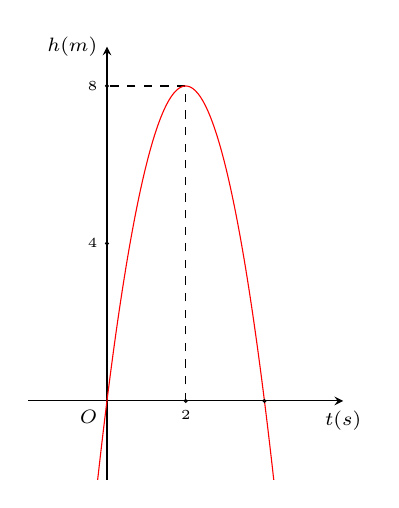
\begin{tikzpicture}[>=stealth,x=1cm,y=1cm,scale=0.5,font=\tiny]
		 \def\a{-2}
		 \def\b{8}
		\def\c{0} 
		\draw[->] (-2,0)  -- (6,0) node[below] {\scriptsize $t (s)$};
		\draw[->] (0,-2) -- (0,9) node[left] {\scriptsize $h (m)$}; 
		\draw  (0,0) node[below left]{\scriptsize $O$};
		\fill (0,4)  node[left]{$4$};
		\fill (0,8) node[left]{$8$}; 
		\fill  (2,0) node[below]{$2$};
		\draw[dashed] (2,0)--(2,8)--(0,8); 
		\pgfmathsetmacro\xdinh{-(\b)/2*(\a)} 
		\pgfmathsetmacro\ydinh{(4*(\a)*(\c)-(\b)^2)/(4*(\a))} 
		\clip  (-2,-2) rectangle (6,9);
		\draw[red,samples=150,smooth,domain=-5:5] plot  (\x,{\a*(\x)^2+(\b)*\x+(\c)});
		\foreach \x in  {2,4} \draw (\x,0) circle (1pt);
		 \foreach \y in {4,8} \draw (0,\y) circle (1pt);
	\end{tikzpicture}
	} 
	\shortans{8} 
	\loigiai{ 
		Hàm số trên là  hàm đa thức nên liên tục trên $\mathbb{R}$.\\
		Dựa vào đồ thị ta có $\displaystyle\lim\limits_{t\to  2}(-2t^{2}+8t)=8$.
	} 
\end{ex}

% nguồn: Ok_TraLoiNgan_Lop11_Lan2
\begin{ex}%[1D3V3-6]%[ma:33e700ce]
	 Hàm số
	$v(t)=\heva{ 
	& -t^2+4 t+12 & \text{khi } 0\leqslant t\leqslant  5\\
	& a t-3 &  \text{khi } 5<t\leqslant 10
	}$ mô tả vận tốc (m/s) của một  vật tại thời điểm $t$ (giây) trong $10$ giây đầu tiên kể từ khi vật bắt đầu chuyển động. Biết rằng $v(t)$ liên tục trên đoạn $[0;10]$ và trong $10$ giây đầu tiên, vật đạt vận tốc $10$ (m/s) đúng hai lần vào các thời điểm $t_1$ và $t_2$. Tính $t_1+t_2$ (làm tròn đến hàng phần chục).
	\shortans{10,9} 
	 \loigiai{
		Hàm số liên tục trên $[0;10]$ nên liên tục tại  $t=5$.
		\begin{eqnarray*}
			&&\lim\limits_{t\to5^+} v(t)=\lim\limits_{t\to5^-} v(t)=v(5)  \\
			&\Rightarrow& \lim\limits_{t\to5^+} (a t-3)=\lim\limits_{t\to5^-} (-t^2+4 t+12)  \\
			&\Rightarrow&  5a-3 = -25+20+12 = 7 \Rightarrow a=2.
		\end{eqnarray*}
		Khi  đó
		 $v(t)=\heva{
		& -t^2+4 t+12 & \text{khi } 0\leqslant t\leqslant 5\\ 
		& 2 t-3 & \text{khi  } 5<t\leqslant 10.
		}$\\ 
		Vật đạt vận  tốc $10$ m/s $\Rightarrow v(t)=10$.\\
		 Suy ra
		 $\heva{
		& -t^2+4 t+12  = 10 & (0\leqslant t\leqslant 5)\\
		& 2 t-3 = 10  & (5<t\leqslant 10)
		 } \Rightarrow \hoac{
		& t=2+\sqrt{6}  \\
		 & t=\dfrac{13}{2}.
		 }$\\
		Vậy $t_1+t_2 =  2+\sqrt{6}+\dfrac{13}{2} \approx 10{,}9$.
	} 
\end{ex}
